%
% teil2.tex -- Beispiel-File für teil2 
%
% (c) 2020 Prof Dr Andreas Müller, Hochschule Rapperswil
%
% !TEX root = ../../buch.tex
% !TEX encoding = UTF-8
%
\section{Riemannsche Zeta-Funktion}\label{Riemannsche Zeta-Funktion}

Die Riemannsche Zeta-Funktion wurde 1859 von Bernhard Riemann untersucht und ist eine zentrale Funktion der
analytischen Zahlentheorie. Sie wird üblicherweise als unendliche Reihe
definiert. Für alle komplexen Variablen s mit Realteil grösser als 1
ergibt sich ihre Darstellung als
\[
\zeta(s) = \sum_{n = 1}^{\infty}\frac{1}{n^{s}}.
\]
Diese Definition beschreibt eine Dirichlet-Reihe, deren Konvergenz für Re(s) \textgreater{} 1 gewährleistet ist. 
Bereits in diesem Definitionsbereich zeigt die Funktion bemerkenswerte Eigenschaften. 
So nimmt sie für bestimmte Argumente konkrete Werte an:

\begin{table}[h]
	\centering
	\begin{tabular}{|c|c|c|}
		\hline
		\rowcolor{blue!40}
		\textcolor{white}{\textbf{\textit{s}}} & 
		\textcolor{white}{\textbf{$\zeta(s)$}} & 
		\textcolor{white}{\textbf{Ungefährer Wert}} \\
		\hline
		$2$ & $\pi^2/6$ & $\approx 1{,}6449$ \\
		\hline
		$4$ & $\pi^4/90$ & $\approx 1{,}0823$ \\
		\hline
		$0$ & $-1/2$ & (analytische Fortsetzung) \\
		\hline
	\end{tabular}
	\caption{Ausgewählte Werte der Zeta-Funktion}
	\label{tab:zeta}
\end{table}

Besonders bemerkenswert ist hier der Wert $\zeta$(2) = $\frac{\pi^2}{6}$, den Euler bereits 1735 nachwies, bekannt als das Basler Problem. 
Die letze Zeile der Tabelle gehört jedoch nicht zum ursprünglichen Definitionsbereich (s > 1), sondern ist nur durch analytische Fortsetzung erreichbar. 

Ein besonders interessanter Fall ist $s = -1$.
Setzt man diesen Wert formal in die Reihendefinition ein, so erhält man
\[
\zeta(-1) \overset{?}{=} \sum_{n=1}^{\infty} \frac{1}{n^{-1}} = \sum_{n=1}^{\infty} n = 1 + 2 + 3 + \ldots,
\]
also genau die Summe aller natürlichen Zahlen.
Dieses Einsetzen ist jedoch nicht zulässig: Die Reihe $\sum_{n=1}^{\infty} n^{-s}$ konvergiert nur für $\operatorname{Re}(s) > 1$, für $s = -1$ ist sie schlicht divergent und die Reihendefinition liefert keinen Wert.
Der Wert von $\zeta(-1)$ kann also nicht direkt aus der Reihe berechnet werden, sondern muss auf anderem Weg gewonnen werden.
Wie dies mit Hilfe der analytischen Fortsetzung gelingt, wird in Abschnitt~\ref{Analytische Fortsetzung} gezeigt.

\begin{figure}
	\centering
	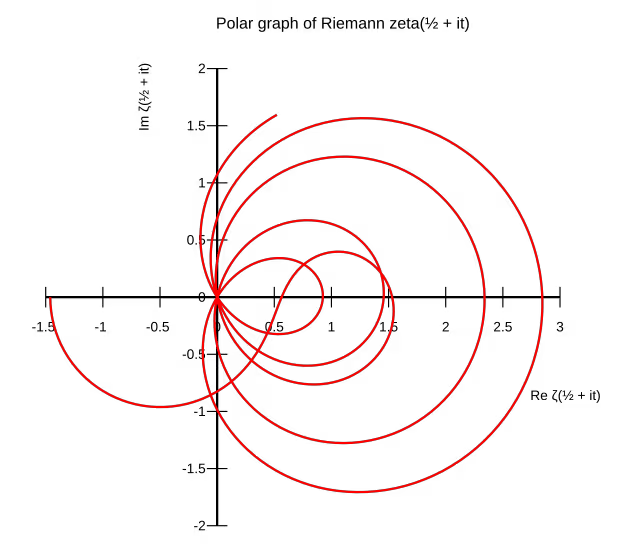
\includegraphics[width=0.7\linewidth]{papers/zeta/Abbildung_Zeta.png}
	\caption{Zeta-Funktion in der komplexen Ebene}
	\label{fig:abbildungzeta}
\end{figure}

Die spiralförmige Darstellung in Abbildung \ref{fig:abbildungzeta} zeigt den Verlauf der Zeta-Funktion $\zeta$(s) in der komplexen Ebene, wobei s entlang einer vertikalen Linie mit festem Realteil variiert. Die Schnittpunkte der Kurve mit dem Ursprung (sichtbar als die Stellen, an denen die Spirale durch den Mittelpunkt verläuft) entsprechen den sogenannten nicht-trivialen Nullstellen der Zeta-Funktion. Diese liegen alle auf der Linie Re(s) = $\frac{1}{2}$ und sind Gegenstand der berühmten, bis heute unbewiesenen Riemannschen Vermutung, einem der bedeutendsten offenen Probleme der Mathematik. 

Nützlich ist die Riemannsche Zeta-Funktion ebenfalls, um eine Annäherung der Primzahlfunktion zu schaffen. 
Das Euler-Produkt
\[
\zeta(s) = \prod_{p \ \text{prim}} \frac{1}{1 - p^{-s}}
\]
beschreibt eine geometrische Reihe,welche den Zusammenhang aller Primzahlen aufzeigt. 

\begin{figure}
	\centering
	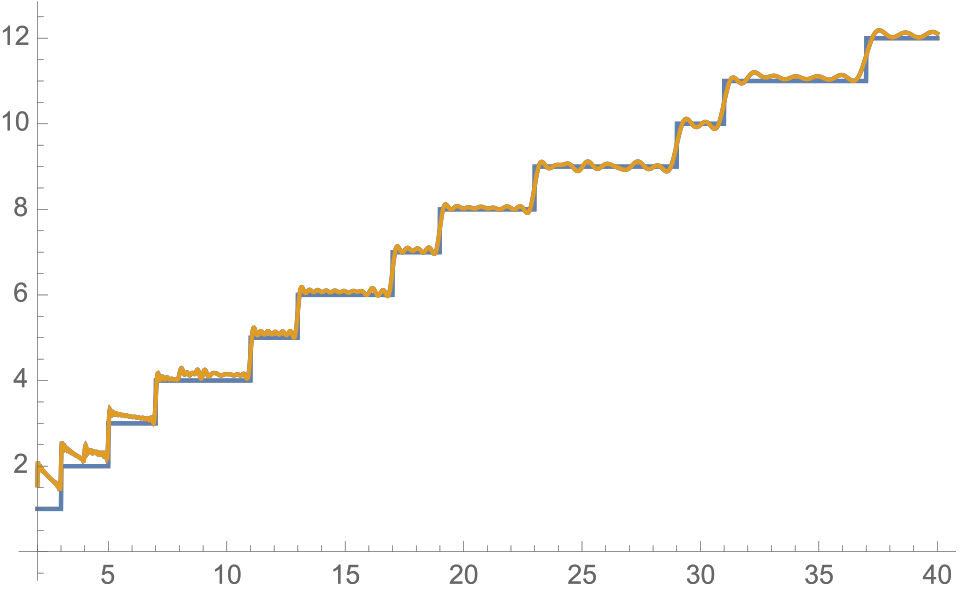
\includegraphics[width=0.7\linewidth]{papers/zeta/Primzahlen.png}
	\caption{Primzahlzählfunktion}
	\label{fig:primzahlen}
\end{figure}

Die blaue Treppenkurve in Abbildung \ref{fig:primzahlen} zeigt die Primzahlzählfunktion $\pi(x)$, welche für jede reelle Zahl $x$ angibt, wie viele Primzahlen kleiner oder gleich $x$ existieren.
Die orangefarbene Kurve stellt den logarithmischen Integralausdruck $\operatorname{Li}(x)$ dar, eine glatte, sprungfreie Funktion.
Das ist eine von Riemann entwickelte Näherungsformel für $\pi(x)$, die direkt aus der Zeta-Funktion abgeleitet wird.
Man erkennt, wie eng beide Kurven beieinander liegen: $\operatorname{Li}(x)$ approximiert die Verteilung der Primzahlen, wobei die relative Genauigkeit dieser Näherung mit wachsendem $x$ zunimmt.

